\documentclass{article}
\usepackage{listings}
\usepackage{mathrsfs}
\usepackage[utf8]{inputenc}
\usepackage{amssymb}
\usepackage{lipsum}
\usepackage{amsmath}
\usepackage{fancyhdr}
\usepackage{geometry}
\usepackage{scrextend}
\usepackage[english,german]{babel}
\usepackage{titling}
\setlength{\droptitle}{-3cm}
\usepackage{tikz}
\usepackage{algorithm,algpseudocode}
\usepackage[doublespacing]{setspace}
\usetikzlibrary{datavisualization}
\usetikzlibrary{datavisualization.formats.functions}
\usepackage{polynom}
\usepackage{amsmath}
\usepackage{gauss}
\usepackage{tkz-euclide}
\usetikzlibrary{datavisualization}
\usetikzlibrary{datavisualization.formats.functions}
\author{
Alexander Mattick Kennung: qi69dube\\
Kapitel 1
}
\usepackage{import}
\date{\today}
\geometry{a4paper, margin=2cm}
\usepackage{stackengine}
\parskip 1em
\newcommand\stackequal[2]{%
  \mathrel{\stackunder[2pt]{\stackon[4pt]{=}{$\scriptscriptstyle#1$}}{%
  $\scriptscriptstyle#2$}}
 }
\makeatletter
\renewcommand*\env@matrix[1][*\c@MaxMatrixCols c]{%
  \hskip -\arraycolsep
  \let\@ifnextchar\new@ifnextchar
  \array{#1}}
\makeatother
\lstset{
  language=haskell,
}
\lstnewenvironment{code}{\lstset{language=Haskell,basicstyle=\small}}{}
\usepackage{enumitem}
\setlist{nosep}
\usepackage{titlesec}
\usepackage{ stmaryrd }
\usepackage{verbatim}


\titlespacing*{\subsection}{0pt}{2pt}{3pt}
\titlespacing*{\section}{0pt}{0pt}{5pt}
\titlespacing*{\subsubsection}{0pt}{1pt}{2pt}
\title{Vorlesung 4}


\begin{document}
	\maketitle
	Faltung zweier Normalverteilungen:\\
	\[X\sim N(a,\sigma^2), Y\sim N(b,\tau^2)\]
	$X+Y = N(a+b, \sigma^2+\tau^2)$\\
	Alternative Notation (mit var stat std)
	\[X\sim N(a,\sigma), Y\sim N(b,\tau)\]
	\[X+Y = N(a+b,\sqrt{\sigma^2+\tau^2})\]
	\section{Zufallsvariable}
	X gehört zu einem Wahrscheinlichkeitsraum $(\Omega,\mathcal{A},P)$
	X ist eine Abbildung $X:(\Omega,\mathcal{A})\to (\Omega',\mathcal{A}')$\\
	mit 
	\[\{X\in A'\}\in\mathcal{A}\forall A'\in\mathcal{A}' = \{\omega\in\Omega|X(\omega)\in A'\}\]
	Frage die gestellt wird $X\sim ?$ Verteilung $\leftrightarrow$ korrespondierende Dichte P.\\
	Oft wird auch die Identität als ZV verwendet
	$Y:(\Omega, \mathcal{A})\to (\Omega,\mathcal{A})$\\
	$P^Y$ ``Brücke'' um aus dem konzept Bildmaß die Notation $Y\sim\dots$ besser zu verstehen.\\
	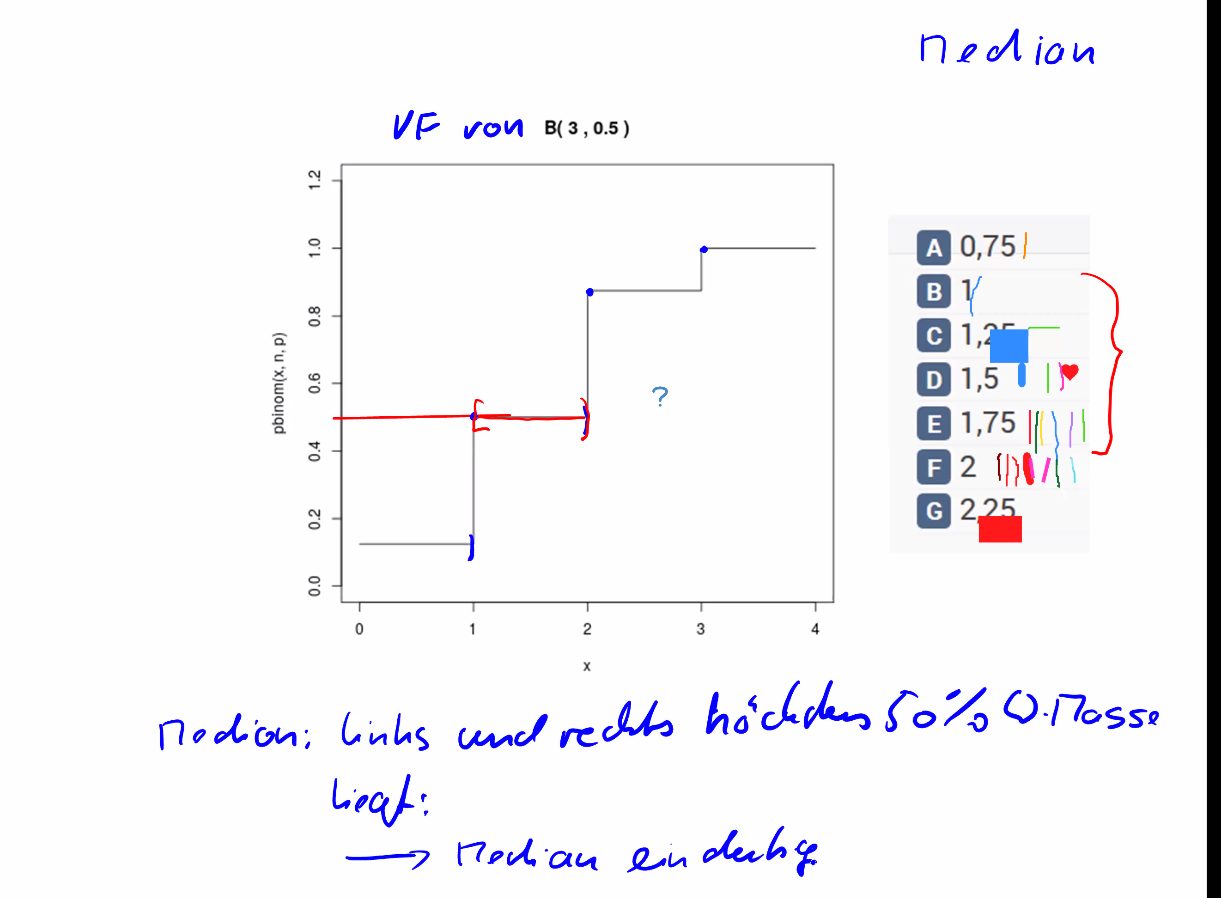
\includegraphics[width=256px]{median.png}
	\\
	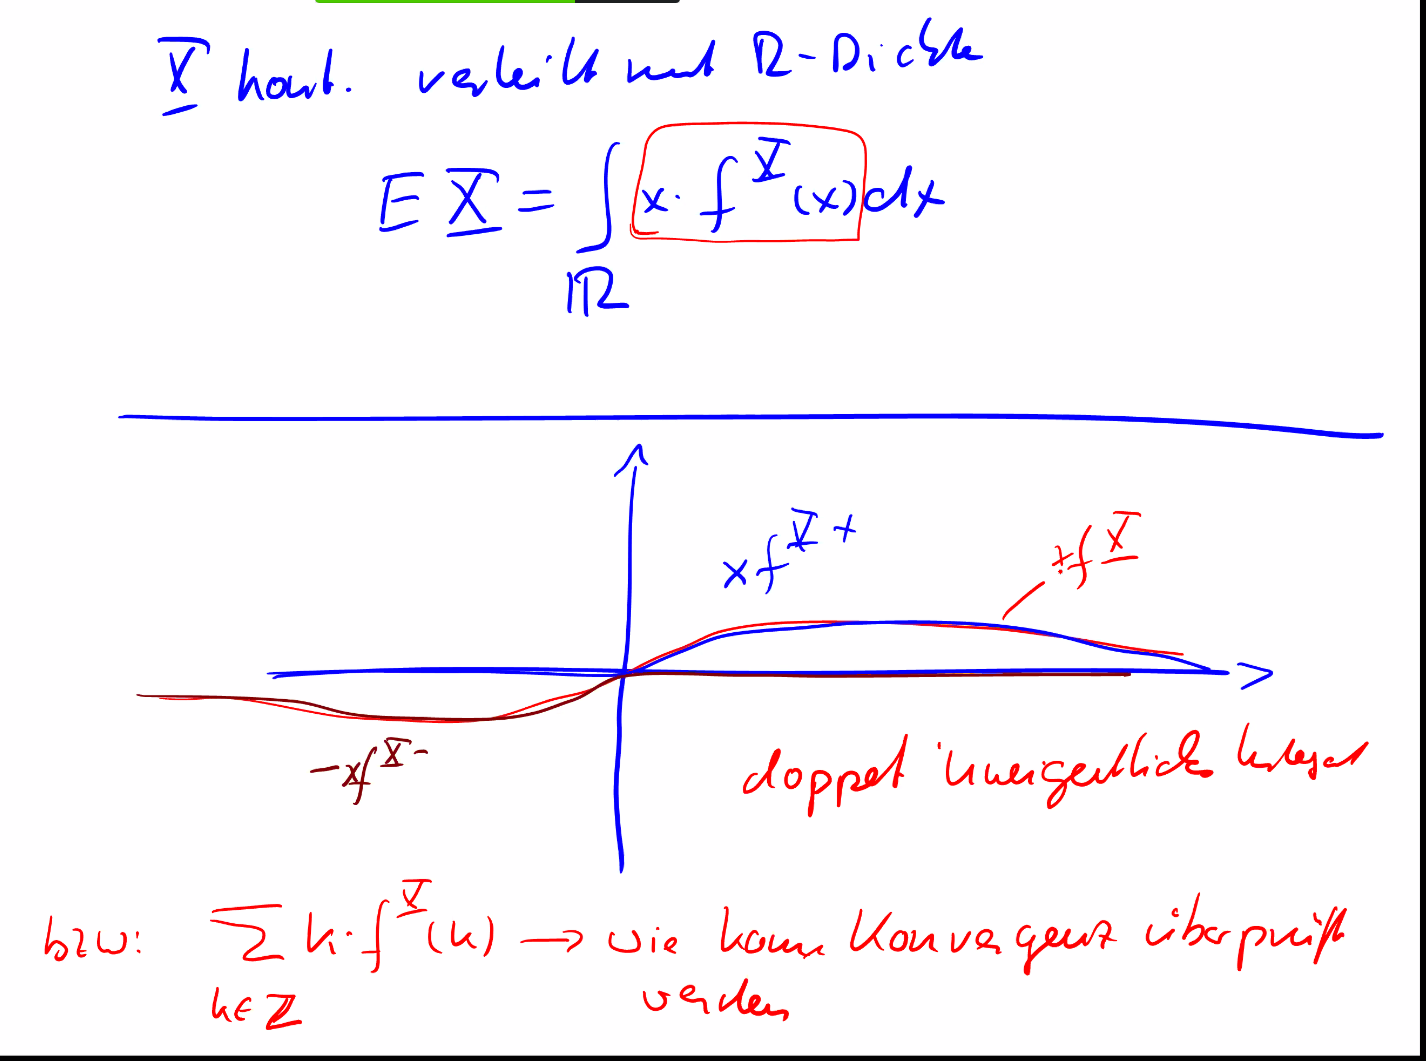
\includegraphics[width=256px]{konvergenz.png}\\
	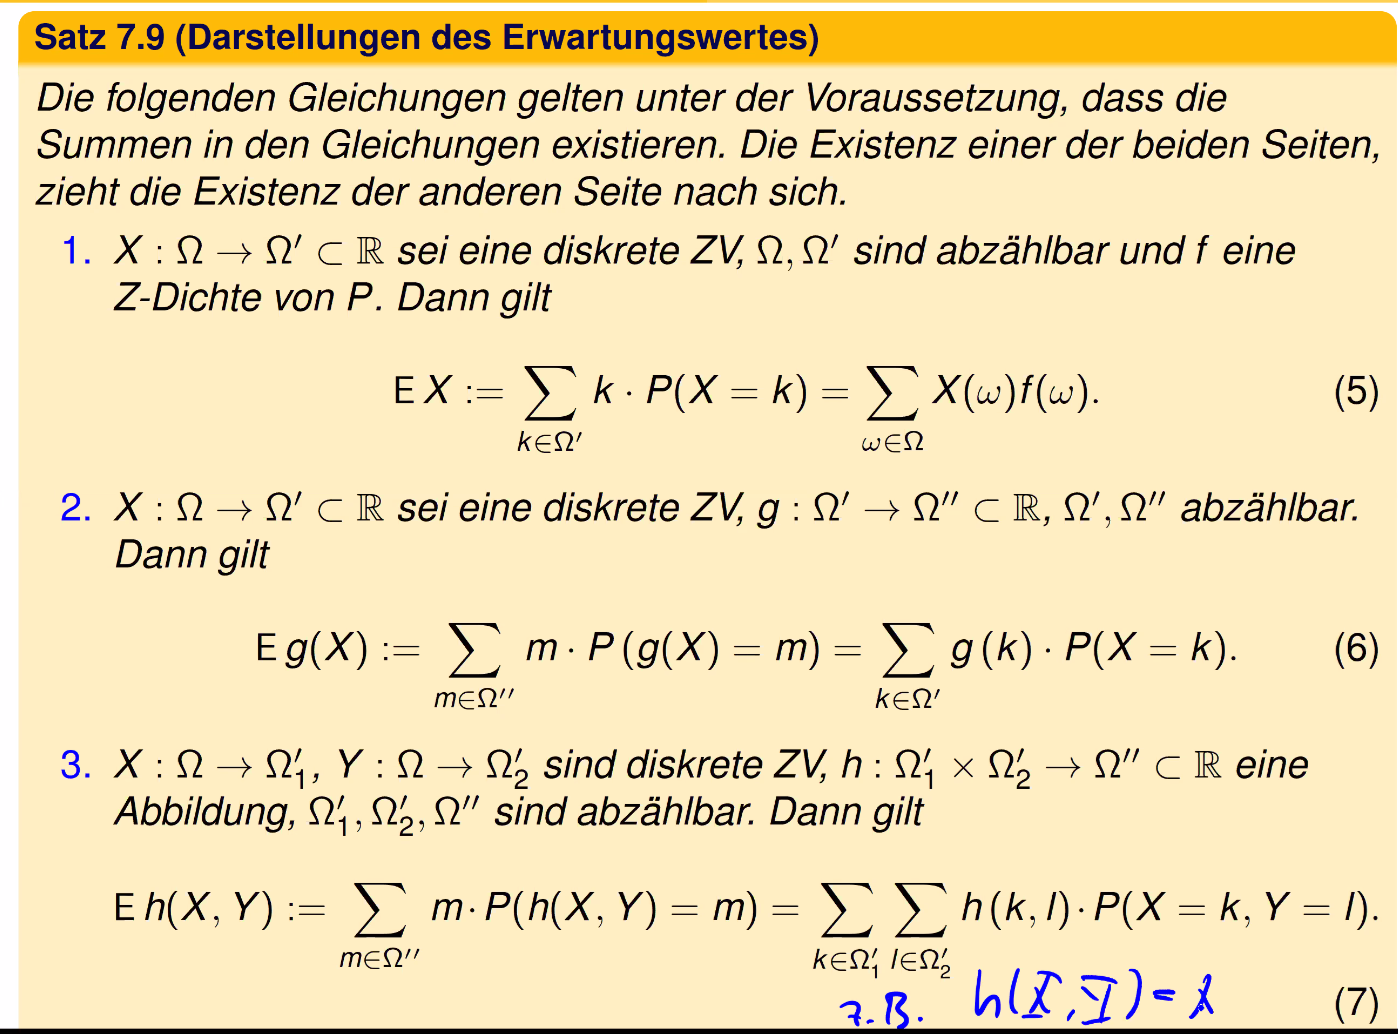
\includegraphics[width=256px]{DarstellungdesErwartungswertes.png}\\
	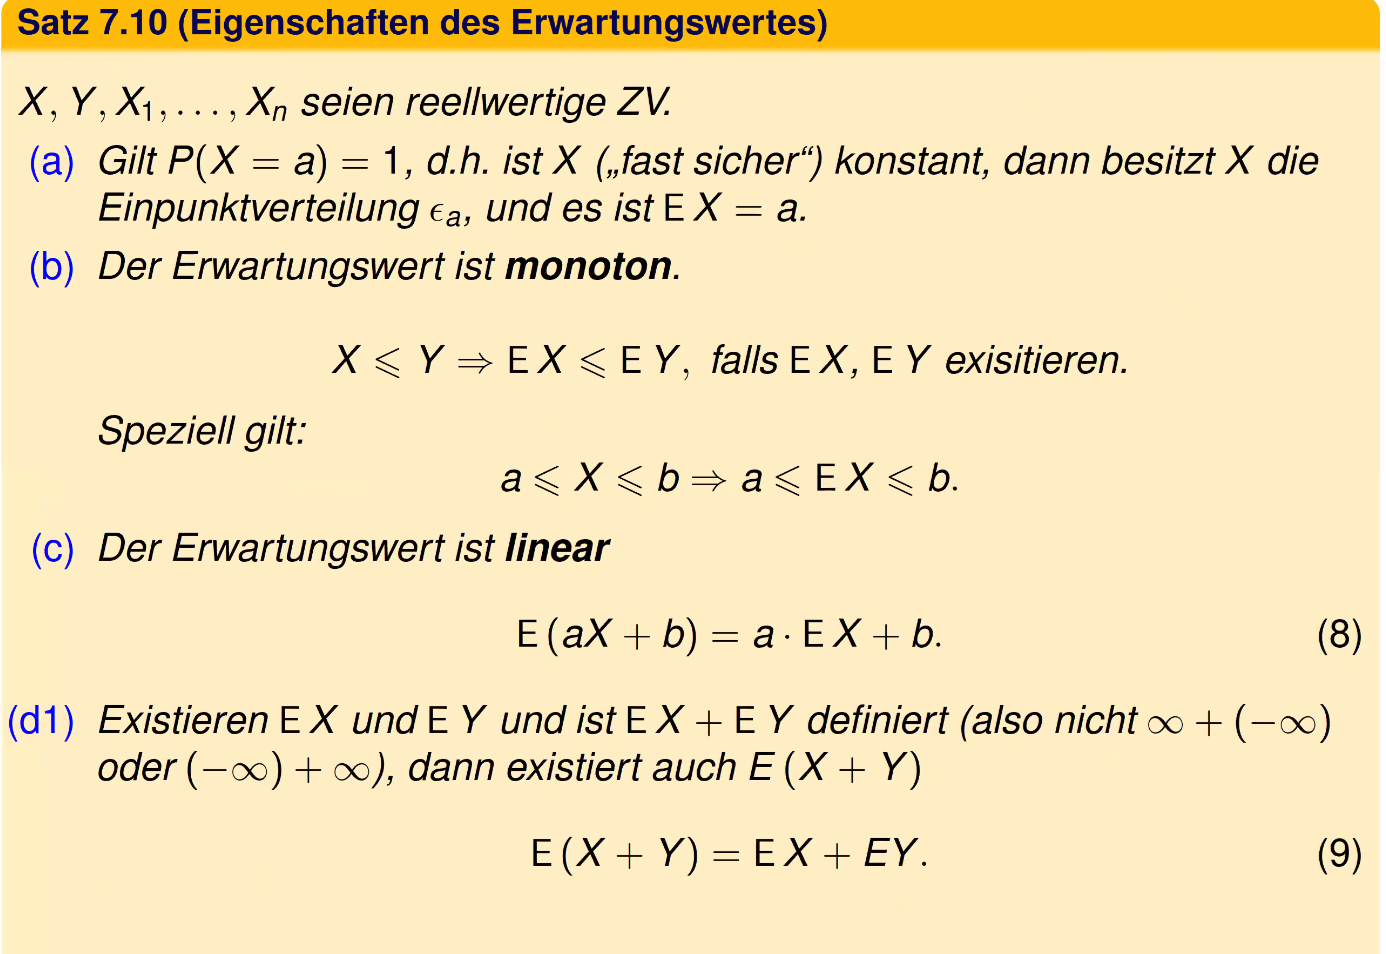
\includegraphics[width=256px]{EigenschaftenvonErwartungswerten.png}\\
	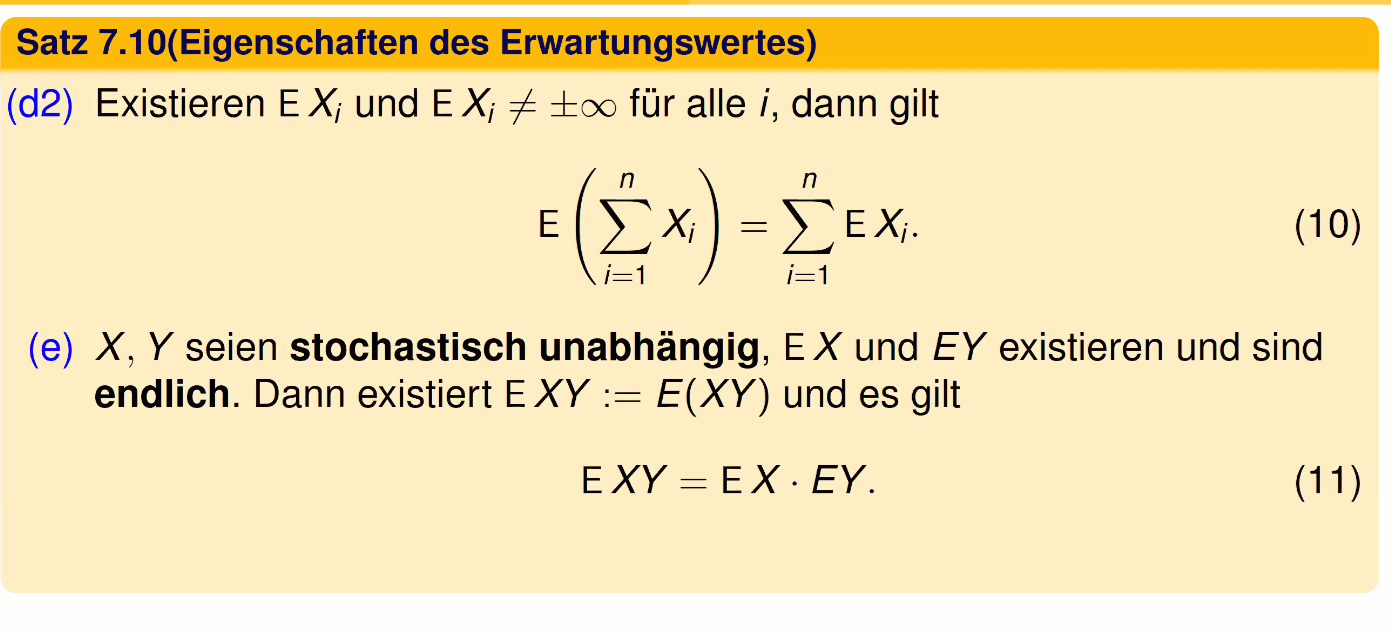
\includegraphics[width=256px]{Eigenschaften2.png}\\
	Daraus folgt die Varianz
	\[var(x) = E(X-Ex)^2 = EX^2-(EX)^2\]
	Für binomialverteilung gilt: $X\sim B(n,p)$	$E X = np$ und $Var(X)=np(1-p)$ \\
	Wenn man das jetzt Normal-approximieren will $Y\sin N(\mu,\sigma^2)$ $E(Y)=\mu, Var(Y)=\sigma^2$
\end{document}